% =====================================================================
%  MSACL DS301 Deep Learning · Quiz 2 · How Networks Learn
%  Academic problem-set style (single-source, \ifsolution toggle)
%  SINGLE SOURCE — produces BOTH the student quiz and the answer key.
%
%  ANSWER TOGGLE
%  -------------
%  Student version (answers HIDDEN) — the default:
%       pdflatex quiz02_training.tex
%  Answer key (answers SHOWN):
%       pdflatex "\def\showsolutions{}% =====================================================================
%  MSACL DS301 Deep Learning · Quiz 2 · How Networks Learn
%  Academic problem-set style (single-source, \ifsolution toggle)
%  SINGLE SOURCE — produces BOTH the student quiz and the answer key.
%
%  ANSWER TOGGLE
%  -------------
%  Student version (answers HIDDEN) — the default:
%       pdflatex quiz02_training.tex
%  Answer key (answers SHOWN):
%       pdflatex "\def\showsolutions{}% =====================================================================
%  MSACL DS301 Deep Learning · Quiz 2 · How Networks Learn
%  Academic problem-set style (single-source, \ifsolution toggle)
%  SINGLE SOURCE — produces BOTH the student quiz and the answer key.
%
%  ANSWER TOGGLE
%  -------------
%  Student version (answers HIDDEN) — the default:
%       pdflatex quiz02_training.tex
%  Answer key (answers SHOWN):
%       pdflatex "\def\showsolutions{}% =====================================================================
%  MSACL DS301 Deep Learning · Quiz 2 · How Networks Learn
%  Academic problem-set style (single-source, \ifsolution toggle)
%  SINGLE SOURCE — produces BOTH the student quiz and the answer key.
%
%  ANSWER TOGGLE
%  -------------
%  Student version (answers HIDDEN) — the default:
%       pdflatex quiz02_training.tex
%  Answer key (answers SHOWN):
%       pdflatex "\def\showsolutions{}\input{quiz02_training.tex}"
%  (or, to flip by hand, change \solutionfalse to \solutiontrue below.)
% =====================================================================
\documentclass[11pt]{article}

\newif\ifsolution
\ifdefined\showsolutions \solutiontrue \else \solutionfalse \fi
% \solutiontrue   % <-- uncomment to hard-code the ANSWER KEY build

\usepackage[letterpaper, margin=0.6in, top=0.7in, bottom=0.5in]{geometry}
\usepackage{amsmath, amssymb}
\usepackage{xcolor}
\usepackage{tikz}
\usepackage{fancyhdr}

\pagestyle{fancy}
\fancyhf{}
\fancyhead[L]{\small\textbf{MSACL DS301 --- Deep Learning}}
\fancyhead[R]{\small\textbf{Quiz 2: How Networks Learn\ifsolution\ \textmd{(Answer Key)}\fi}}
\fancyfoot[C]{\thepage}
\renewcommand{\headrulewidth}{0.4pt}

\newcommand{\blk}[1]{\underline{\hspace{#1}}}
% Reveal-or-blank: shows the answer in the key, a blank rule on the student sheet.
\newcommand{\rb}[2]{\ifsolution\textbf{#1}\else\blk{#2}\fi}
% Boxed answer (key only) and blank writing space (student only).
\newcommand{\keybox}[1]{\ifsolution\par\vspace{2pt}%
  \fbox{\parbox{0.965\textwidth}{\small\textbf{Answer.}\; #1}}\par\fi}
\newcommand{\work}[1]{\ifsolution\else\vspace{#1}\fi}

\setlength{\parindent}{0pt}
\setlength{\parskip}{3pt}
\setlength{\abovedisplayskip}{5pt}
\setlength{\belowdisplayskip}{5pt}

\begin{document}

\begin{center}
{\Large \textbf{Quiz 2 --- How Networks Learn}}\\[2pt]
{\normalsize Loss, backpropagation, one gradient-descent step, and the training loop}
\end{center}

\vspace{-2pt}
\begin{center}
\fbox{\parbox{0.92\textwidth}{\small
\textbf{Instructions:}\; Answer all five questions. Intuition first, light arithmetic ---
show your work on the blanks. No calculators needed.%
\ifsolution\else\\[4pt]\textbf{Name:}\ \blk{6cm}\hfill\textbf{Date:}\ \blk{3.5cm}\fi
}}
\end{center}

\vspace{-2pt}\hrule\vspace{5pt}

% =========================== Q1 ===========================
\textbf{1. Backpropagation on a two-weight network.}\; {\small Same tiny net as the worked
example: one input, one hidden neuron (ReLU), one output --- just two weights.}

\vspace{2pt}
\begin{center}
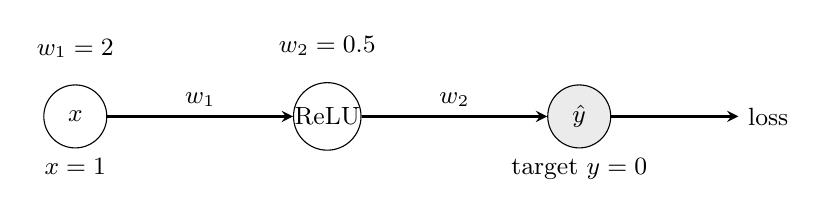
\begin{tikzpicture}[x=1.6cm, y=1cm,
  n/.style={circle, draw, minimum size=8mm, inner sep=0pt, font=\small}, >=stealth]
  \node[n] (x) at (0,0) {$x$};
  \node[n] (h) at (2,0) {ReLU};
  \node[n, fill=black!8] (y) at (4,0) {$\hat y$};
  \node[font=\small] (L) at (5.5,0) {loss};
  \draw[->, thick] (x)--node[above,font=\small]{$w_1$}(h);
  \draw[->, thick] (h)--node[above,font=\small]{$w_2$}(y);
  \draw[->, thick] (y)--(L);
  \node[below, font=\small] at (x.south) {$x=1$};
  \node[above=6pt, font=\small] at (x.north) {$w_1=2$};
  \node[above=6pt, font=\small] at (h.north) {$w_2=0.5$};
  \node[below, font=\small] at (y.south) {target $y=0$};
\end{tikzpicture}
\end{center}

\textbf{(a) Forward pass.}\; {\small Fill in each value, then square the error to get the loss.}
\begin{align*}
h &= \operatorname{ReLU}(w_1 \cdot x) = \operatorname{ReLU}(2 \times 1) = \rb{$2$}{1.4cm}
&\hat y &= w_2 \cdot h = 0.5 \times \rb{$2$}{1cm} = \rb{$1$}{1.4cm}\\[3pt]
\text{error} &= \hat y - y = \rb{$1$}{1.4cm}
&\text{loss} &= (\text{error})^2 = \rb{$1$}{1.4cm}
\end{align*}

\work{0.4cm}

\keybox{$h=\operatorname{ReLU}(2)=2$; \ $\hat y = 0.5\times 2 = 1$; \ error $=1-0=1$; \
loss $=1^2 = 1$. The guess overshot the target of $0$.}

\vspace{4pt}
\textbf{(b) Backward pass --- multiply the local effects along the path.}\;
{\small Recipe from lecture: start with the ``how wrong'' signal $=2\times\text{error}$, then
multiply the local effect at each arrow back to the weight. (The ReLU slope is $1$ because the
hidden value is positive.)}

\vspace{3pt}
``how wrong'' signal $= 2 \times \text{error} = 2 \times 1 = \rb{$2$}{1.4cm}$

\[
\text{gradient of } w_2 \;=\; (2\times\text{error}) \times h
\;=\; \blk{2.4cm} \;=\; \rb{$4$}{1.4cm}
\]
\[
\text{gradient of } w_1 \;=\; (2\times\text{error}) \times w_2 \times (\text{ReLU slope}) \times x
\;=\; \blk{3.6cm} \;=\; \rb{$1$}{1.4cm}
\]

\work{0.6cm}

\keybox{The shared ``how wrong'' signal is $2\times\text{error}=2\times 1 = 2$.\\
gradient of $w_2 = 2 \times h = 2 \times 2 = \mathbf{4}$ \ (short path: only the last weight).\\
gradient of $w_1 = 2 \times w_2 \times 1 \times x = 2 \times 0.5 \times 1 \times 1 = \mathbf{1}$
\ (longer path: back through $w_2$ and the ReLU). Both gradients are positive, so both weights
should decrease.}

\vspace{2pt}\hrule\vspace{5pt}

% =========================== Q2 ===========================
\textbf{2. One gradient-descent step by hand.}\; {\small Use your gradients from Q1 and the
update rule} $\text{new weight} = \text{weight} - \text{lr}\times\text{gradient}$, {\small with
learning rate lr $=0.1$.}

\[
w_2 \leftarrow 0.5 - 0.1 \times \rb{$4$}{1cm} = \rb{$0.1$}{1.6cm}
\qquad\qquad
w_1 \leftarrow 2 - 0.1 \times \rb{$1$}{1cm} = \rb{$1.9$}{1.6cm}
\]

\work{0.7cm}

\keybox{$w_2 \leftarrow 0.5 - 0.1\times 4 = 0.5 - 0.4 = \mathbf{0.1}$; \quad
$w_1 \leftarrow 2 - 0.1\times 1 = 2 - 0.1 = \mathbf{1.9}$. Both came down, as expected --- the
guess was too high. (Re-running the forward pass with the new weights gives loss $\approx 0.04$,
down from $1$: one step already helped.)}

\vspace{2pt}\hrule\vspace{5pt}

% =========================== Q3 ===========================
\textbf{3. Diagnose the loss curve --- and prescribe the fix.}\; {\small For each run, write the
\emph{diagnosis} and the \emph{one change} you would make, using the word banks. Each plot is loss
(vertical) vs.\ epoch (horizontal). Note that (a) and (d) are \textbf{not} the same problem.}

\vspace{4pt}
\begin{center}
\newcommand{\lossaxes}{\draw[->,gray] (0,0)--(3.1,0); \draw[->,gray] (0,0)--(0,2.4);}
%
\begin{minipage}[t]{0.235\linewidth}\centering
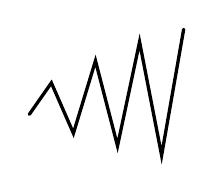
\begin{tikzpicture}[scale=0.8, line cap=round]
  \lossaxes
  \draw[very thick] (0.15,1.0)--(0.5,1.5)--(0.85,0.7)--(1.2,1.85)--(1.55,0.5)--(1.9,2.15)--(2.25,0.35)--(2.6,2.35);
\end{tikzpicture}\\[2pt]
{\footnotesize (a)}\\[3pt]
{\scriptsize diag:}\;\rb{far too high}{1.5cm}\\[4pt]
{\scriptsize fix:}\;\rb{lower a lot}{1.5cm}
\end{minipage}\hfill
%
\begin{minipage}[t]{0.235\linewidth}\centering
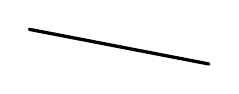
\begin{tikzpicture}[scale=0.8, line cap=round]
  \lossaxes
  \draw[very thick] (0.1,2.05)--(2.95,1.5);
\end{tikzpicture}\\[2pt]
{\footnotesize (b)}\\[3pt]
{\scriptsize diag:}\;\rb{too low}{1.5cm}\\[4pt]
{\scriptsize fix:}\;\rb{raise it}{1.5cm}
\end{minipage}\hfill
%
\begin{minipage}[t]{0.235\linewidth}\centering
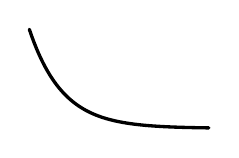
\begin{tikzpicture}[scale=0.8, line cap=round]
  \lossaxes
  \draw[very thick, samples=80, domain=0.1:2.95] plot (\x,{0.35+1.9*exp(-1.9*\x)});
\end{tikzpicture}\\[2pt]
{\footnotesize (c)}\\[3pt]
{\scriptsize diag:}\;\rb{just right}{1.5cm}\\[4pt]
{\scriptsize fix:}\;\rb{keep it}{1.5cm}
\end{minipage}\hfill
%
\begin{minipage}[t]{0.235\linewidth}\centering
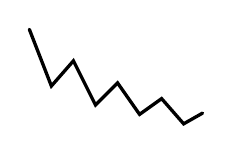
\begin{tikzpicture}[scale=0.8, line cap=round]
  \lossaxes
  \draw[very thick] (0.15,2.05)--(0.5,1.15)--(0.85,1.55)--(1.2,0.85)--(1.55,1.2)--(1.9,0.7)--(2.25,0.95)--(2.6,0.55)--(2.9,0.72);
\end{tikzpicture}\\[2pt]
{\footnotesize (d)}\\[3pt]
{\scriptsize diag:}\;\rb{a bit high}{1.5cm}\\[4pt]
{\scriptsize fix:}\;\rb{lower a little}{1.5cm}
\end{minipage}
\end{center}

\vspace{2pt}
\begin{center}
{\small \textbf{Diagnosis bank:}\;\; far too high (diverging) \;$\cdot$\; a bit too high (noisy but
converging) \;$\cdot$\; too low \;$\cdot$\; just right \\[2pt]
\textbf{Fix bank:}\;\; lower the rate a lot \;$\cdot$\; lower it a little \;$\cdot$\; raise it
\;$\cdot$\; keep it (train longer)}
\end{center}

\keybox{(a) \textbf{far too high $\rightarrow$ lower the rate a lot}: the swings \emph{grow} and the
loss climbs --- the steps overshoot so badly training is diverging. (b) \textbf{too low
$\rightarrow$ raise it}: the loss barely drops and is still high and still falling at the end;
it would get there eventually but wastes time. (c) \textbf{just right $\rightarrow$ keep it}: a
steep early drop that flattens out low and stays there. (d) \textbf{a bit too high $\rightarrow$
lower it a little}: the loss \emph{is} trending down but bounces noisily on the way --- close to
right, just overshooting slightly. The tell that separates (a) from (d): in (a) the swings grow
and the loss rises; in (d) they shrink and the loss falls.}

\vspace{2pt}\hrule\vspace{5pt}

% =========================== Q4 ===========================
\textbf{4. Spot the bug.}\; {\small A colleague's training loop runs with no error, but the loss
\emph{never drops} --- the weights never change at all. All five lines are present, in this order:}

\vspace{4pt}
\begin{center}
\begin{tabular}{@{}l@{\qquad}p{0.40\textwidth}@{}}
\texttt{for x, y in loader:}        & {\small\itshape every batch} \\[4pt]
\hspace{1em}\texttt{pred = model(x)}         & {\small\itshape forward} \\[4pt]
\hspace{1em}\texttt{loss = loss\_fn(pred, y)} & {\small\itshape how wrong?} \\[4pt]
\hspace{1em}\texttt{loss.backward()}          & {\small\itshape backprop the blame} \\[4pt]
\hspace{1em}\texttt{optimizer.zero\_grad()}   & {\small\itshape clear gradients} \\[4pt]
\hspace{1em}\texttt{optimizer.step()}         & {\small\itshape nudge every weight} \\
\end{tabular}
\end{center}

{\small (i) Which line is in the \textbf{wrong place}?}\; \rb{\texttt{optimizer.zero\_grad()}}{6cm}\\[4pt]
{\small (ii) Why does that stop learning, and where should it go?}

\work{0.5cm}

\keybox{(i) \texttt{optimizer.zero\_grad()} is misplaced --- it runs \emph{after}
\texttt{loss.backward()}. (ii) \texttt{backward()} computes this batch's gradients and stores them in
each weight's \texttt{.grad}; \texttt{zero\_grad()} then immediately \textbf{erases} them, so
\texttt{optimizer.step()} applies all-zero gradients and no weight moves --- the loss stays flat
forever. Move \texttt{zero\_grad()} to \emph{before} \texttt{backward()} (correct order:
\texttt{zero\_grad} $\rightarrow$ \texttt{backward} $\rightarrow$ \texttt{step}). Gradients live in
\texttt{.grad} and must be cleared just \emph{before}, never just after, the backward sweep.}

% =========================== Q5 ===========================
\textbf{5. Looking ahead (discussion).}\; {\small A short thought question --- one or two sentences
each. This one previews a later lecture, so reason it out rather than compute.}

\vspace{3pt}
You train a network and watch the loss on your \emph{training} samples fall steadily, almost to
zero --- the model gets the training data nearly perfect. But when you score it on a batch of
\emph{fresh, held-out} samples it has never seen, the loss stops improving and then starts to
\emph{rise}.

\vspace{4pt}
(a) What might be going wrong? \hfill (b) Does a lower training loss always mean a better model?

\work{1.6cm}
\ifsolution\else\blk{\linewidth}\\[10pt]\blk{\linewidth}\\[10pt]\blk{\linewidth}\fi

\keybox{(a) This is \textbf{overfitting}: the network is starting to \emph{memorise} the quirks and
noise of the training set instead of learning the general pattern, so it keeps improving on seen
data while getting worse on new data. (b) \textbf{No.} A lower \emph{training} loss does not mean a
better model --- what matters is performance on \emph{unseen} data (generalisation); once the two
curves split apart, more training makes the model worse in practice. (Lecture 4 names the fixes:
more/cleaner data, regularisation, dropout, and early stopping --- stop where the held-out loss
turns up.)}

\vspace{4pt}\hrule\vspace{3pt}
{\small\itshape \ifsolution Answer key.\else Keep this sheet --- the backprop recipe and the
five-line loop are your Lab 1 cheat-sheet.\fi}

\end{document}
"
%  (or, to flip by hand, change \solutionfalse to \solutiontrue below.)
% =====================================================================
\documentclass[11pt]{article}

\newif\ifsolution
\ifdefined\showsolutions \solutiontrue \else \solutionfalse \fi
% \solutiontrue   % <-- uncomment to hard-code the ANSWER KEY build

\usepackage[letterpaper, margin=0.6in, top=0.7in, bottom=0.5in]{geometry}
\usepackage{amsmath, amssymb}
\usepackage{xcolor}
\usepackage{tikz}
\usepackage{fancyhdr}

\pagestyle{fancy}
\fancyhf{}
\fancyhead[L]{\small\textbf{MSACL DS301 --- Deep Learning}}
\fancyhead[R]{\small\textbf{Quiz 2: How Networks Learn\ifsolution\ \textmd{(Answer Key)}\fi}}
\fancyfoot[C]{\thepage}
\renewcommand{\headrulewidth}{0.4pt}

\newcommand{\blk}[1]{\underline{\hspace{#1}}}
% Reveal-or-blank: shows the answer in the key, a blank rule on the student sheet.
\newcommand{\rb}[2]{\ifsolution\textbf{#1}\else\blk{#2}\fi}
% Boxed answer (key only) and blank writing space (student only).
\newcommand{\keybox}[1]{\ifsolution\par\vspace{2pt}%
  \fbox{\parbox{0.965\textwidth}{\small\textbf{Answer.}\; #1}}\par\fi}
\newcommand{\work}[1]{\ifsolution\else\vspace{#1}\fi}

\setlength{\parindent}{0pt}
\setlength{\parskip}{3pt}
\setlength{\abovedisplayskip}{5pt}
\setlength{\belowdisplayskip}{5pt}

\begin{document}

\begin{center}
{\Large \textbf{Quiz 2 --- How Networks Learn}}\\[2pt]
{\normalsize Loss, backpropagation, one gradient-descent step, and the training loop}
\end{center}

\vspace{-2pt}
\begin{center}
\fbox{\parbox{0.92\textwidth}{\small
\textbf{Instructions:}\; Answer all five questions. Intuition first, light arithmetic ---
show your work on the blanks. No calculators needed.%
\ifsolution\else\\[4pt]\textbf{Name:}\ \blk{6cm}\hfill\textbf{Date:}\ \blk{3.5cm}\fi
}}
\end{center}

\vspace{-2pt}\hrule\vspace{5pt}

% =========================== Q1 ===========================
\textbf{1. Backpropagation on a two-weight network.}\; {\small Same tiny net as the worked
example: one input, one hidden neuron (ReLU), one output --- just two weights.}

\vspace{2pt}
\begin{center}
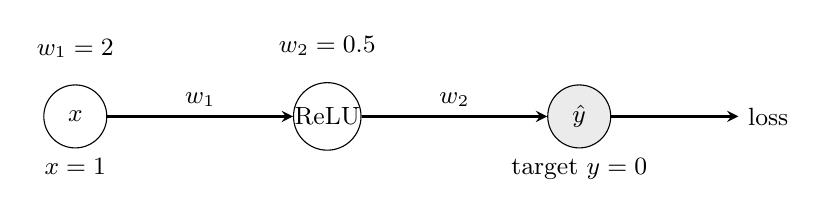
\begin{tikzpicture}[x=1.6cm, y=1cm,
  n/.style={circle, draw, minimum size=8mm, inner sep=0pt, font=\small}, >=stealth]
  \node[n] (x) at (0,0) {$x$};
  \node[n] (h) at (2,0) {ReLU};
  \node[n, fill=black!8] (y) at (4,0) {$\hat y$};
  \node[font=\small] (L) at (5.5,0) {loss};
  \draw[->, thick] (x)--node[above,font=\small]{$w_1$}(h);
  \draw[->, thick] (h)--node[above,font=\small]{$w_2$}(y);
  \draw[->, thick] (y)--(L);
  \node[below, font=\small] at (x.south) {$x=1$};
  \node[above=6pt, font=\small] at (x.north) {$w_1=2$};
  \node[above=6pt, font=\small] at (h.north) {$w_2=0.5$};
  \node[below, font=\small] at (y.south) {target $y=0$};
\end{tikzpicture}
\end{center}

\textbf{(a) Forward pass.}\; {\small Fill in each value, then square the error to get the loss.}
\begin{align*}
h &= \operatorname{ReLU}(w_1 \cdot x) = \operatorname{ReLU}(2 \times 1) = \rb{$2$}{1.4cm}
&\hat y &= w_2 \cdot h = 0.5 \times \rb{$2$}{1cm} = \rb{$1$}{1.4cm}\\[3pt]
\text{error} &= \hat y - y = \rb{$1$}{1.4cm}
&\text{loss} &= (\text{error})^2 = \rb{$1$}{1.4cm}
\end{align*}

\work{0.4cm}

\keybox{$h=\operatorname{ReLU}(2)=2$; \ $\hat y = 0.5\times 2 = 1$; \ error $=1-0=1$; \
loss $=1^2 = 1$. The guess overshot the target of $0$.}

\vspace{4pt}
\textbf{(b) Backward pass --- multiply the local effects along the path.}\;
{\small Recipe from lecture: start with the ``how wrong'' signal $=2\times\text{error}$, then
multiply the local effect at each arrow back to the weight. (The ReLU slope is $1$ because the
hidden value is positive.)}

\vspace{3pt}
``how wrong'' signal $= 2 \times \text{error} = 2 \times 1 = \rb{$2$}{1.4cm}$

\[
\text{gradient of } w_2 \;=\; (2\times\text{error}) \times h
\;=\; \blk{2.4cm} \;=\; \rb{$4$}{1.4cm}
\]
\[
\text{gradient of } w_1 \;=\; (2\times\text{error}) \times w_2 \times (\text{ReLU slope}) \times x
\;=\; \blk{3.6cm} \;=\; \rb{$1$}{1.4cm}
\]

\work{0.6cm}

\keybox{The shared ``how wrong'' signal is $2\times\text{error}=2\times 1 = 2$.\\
gradient of $w_2 = 2 \times h = 2 \times 2 = \mathbf{4}$ \ (short path: only the last weight).\\
gradient of $w_1 = 2 \times w_2 \times 1 \times x = 2 \times 0.5 \times 1 \times 1 = \mathbf{1}$
\ (longer path: back through $w_2$ and the ReLU). Both gradients are positive, so both weights
should decrease.}

\vspace{2pt}\hrule\vspace{5pt}

% =========================== Q2 ===========================
\textbf{2. One gradient-descent step by hand.}\; {\small Use your gradients from Q1 and the
update rule} $\text{new weight} = \text{weight} - \text{lr}\times\text{gradient}$, {\small with
learning rate lr $=0.1$.}

\[
w_2 \leftarrow 0.5 - 0.1 \times \rb{$4$}{1cm} = \rb{$0.1$}{1.6cm}
\qquad\qquad
w_1 \leftarrow 2 - 0.1 \times \rb{$1$}{1cm} = \rb{$1.9$}{1.6cm}
\]

\work{0.7cm}

\keybox{$w_2 \leftarrow 0.5 - 0.1\times 4 = 0.5 - 0.4 = \mathbf{0.1}$; \quad
$w_1 \leftarrow 2 - 0.1\times 1 = 2 - 0.1 = \mathbf{1.9}$. Both came down, as expected --- the
guess was too high. (Re-running the forward pass with the new weights gives loss $\approx 0.04$,
down from $1$: one step already helped.)}

\vspace{2pt}\hrule\vspace{5pt}

% =========================== Q3 ===========================
\textbf{3. Diagnose the loss curve --- and prescribe the fix.}\; {\small For each run, write the
\emph{diagnosis} and the \emph{one change} you would make, using the word banks. Each plot is loss
(vertical) vs.\ epoch (horizontal). Note that (a) and (d) are \textbf{not} the same problem.}

\vspace{4pt}
\begin{center}
\newcommand{\lossaxes}{\draw[->,gray] (0,0)--(3.1,0); \draw[->,gray] (0,0)--(0,2.4);}
%
\begin{minipage}[t]{0.235\linewidth}\centering
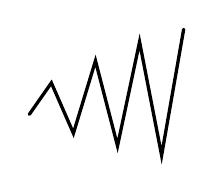
\begin{tikzpicture}[scale=0.8, line cap=round]
  \lossaxes
  \draw[very thick] (0.15,1.0)--(0.5,1.5)--(0.85,0.7)--(1.2,1.85)--(1.55,0.5)--(1.9,2.15)--(2.25,0.35)--(2.6,2.35);
\end{tikzpicture}\\[2pt]
{\footnotesize (a)}\\[3pt]
{\scriptsize diag:}\;\rb{far too high}{1.5cm}\\[4pt]
{\scriptsize fix:}\;\rb{lower a lot}{1.5cm}
\end{minipage}\hfill
%
\begin{minipage}[t]{0.235\linewidth}\centering
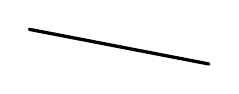
\begin{tikzpicture}[scale=0.8, line cap=round]
  \lossaxes
  \draw[very thick] (0.1,2.05)--(2.95,1.5);
\end{tikzpicture}\\[2pt]
{\footnotesize (b)}\\[3pt]
{\scriptsize diag:}\;\rb{too low}{1.5cm}\\[4pt]
{\scriptsize fix:}\;\rb{raise it}{1.5cm}
\end{minipage}\hfill
%
\begin{minipage}[t]{0.235\linewidth}\centering
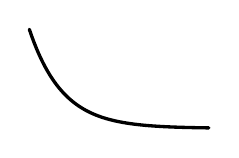
\begin{tikzpicture}[scale=0.8, line cap=round]
  \lossaxes
  \draw[very thick, samples=80, domain=0.1:2.95] plot (\x,{0.35+1.9*exp(-1.9*\x)});
\end{tikzpicture}\\[2pt]
{\footnotesize (c)}\\[3pt]
{\scriptsize diag:}\;\rb{just right}{1.5cm}\\[4pt]
{\scriptsize fix:}\;\rb{keep it}{1.5cm}
\end{minipage}\hfill
%
\begin{minipage}[t]{0.235\linewidth}\centering
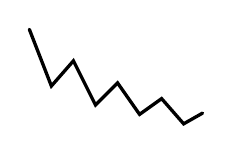
\begin{tikzpicture}[scale=0.8, line cap=round]
  \lossaxes
  \draw[very thick] (0.15,2.05)--(0.5,1.15)--(0.85,1.55)--(1.2,0.85)--(1.55,1.2)--(1.9,0.7)--(2.25,0.95)--(2.6,0.55)--(2.9,0.72);
\end{tikzpicture}\\[2pt]
{\footnotesize (d)}\\[3pt]
{\scriptsize diag:}\;\rb{a bit high}{1.5cm}\\[4pt]
{\scriptsize fix:}\;\rb{lower a little}{1.5cm}
\end{minipage}
\end{center}

\vspace{2pt}
\begin{center}
{\small \textbf{Diagnosis bank:}\;\; far too high (diverging) \;$\cdot$\; a bit too high (noisy but
converging) \;$\cdot$\; too low \;$\cdot$\; just right \\[2pt]
\textbf{Fix bank:}\;\; lower the rate a lot \;$\cdot$\; lower it a little \;$\cdot$\; raise it
\;$\cdot$\; keep it (train longer)}
\end{center}

\keybox{(a) \textbf{far too high $\rightarrow$ lower the rate a lot}: the swings \emph{grow} and the
loss climbs --- the steps overshoot so badly training is diverging. (b) \textbf{too low
$\rightarrow$ raise it}: the loss barely drops and is still high and still falling at the end;
it would get there eventually but wastes time. (c) \textbf{just right $\rightarrow$ keep it}: a
steep early drop that flattens out low and stays there. (d) \textbf{a bit too high $\rightarrow$
lower it a little}: the loss \emph{is} trending down but bounces noisily on the way --- close to
right, just overshooting slightly. The tell that separates (a) from (d): in (a) the swings grow
and the loss rises; in (d) they shrink and the loss falls.}

\vspace{2pt}\hrule\vspace{5pt}

% =========================== Q4 ===========================
\textbf{4. Spot the bug.}\; {\small A colleague's training loop runs with no error, but the loss
\emph{never drops} --- the weights never change at all. All five lines are present, in this order:}

\vspace{4pt}
\begin{center}
\begin{tabular}{@{}l@{\qquad}p{0.40\textwidth}@{}}
\texttt{for x, y in loader:}        & {\small\itshape every batch} \\[4pt]
\hspace{1em}\texttt{pred = model(x)}         & {\small\itshape forward} \\[4pt]
\hspace{1em}\texttt{loss = loss\_fn(pred, y)} & {\small\itshape how wrong?} \\[4pt]
\hspace{1em}\texttt{loss.backward()}          & {\small\itshape backprop the blame} \\[4pt]
\hspace{1em}\texttt{optimizer.zero\_grad()}   & {\small\itshape clear gradients} \\[4pt]
\hspace{1em}\texttt{optimizer.step()}         & {\small\itshape nudge every weight} \\
\end{tabular}
\end{center}

{\small (i) Which line is in the \textbf{wrong place}?}\; \rb{\texttt{optimizer.zero\_grad()}}{6cm}\\[4pt]
{\small (ii) Why does that stop learning, and where should it go?}

\work{0.5cm}

\keybox{(i) \texttt{optimizer.zero\_grad()} is misplaced --- it runs \emph{after}
\texttt{loss.backward()}. (ii) \texttt{backward()} computes this batch's gradients and stores them in
each weight's \texttt{.grad}; \texttt{zero\_grad()} then immediately \textbf{erases} them, so
\texttt{optimizer.step()} applies all-zero gradients and no weight moves --- the loss stays flat
forever. Move \texttt{zero\_grad()} to \emph{before} \texttt{backward()} (correct order:
\texttt{zero\_grad} $\rightarrow$ \texttt{backward} $\rightarrow$ \texttt{step}). Gradients live in
\texttt{.grad} and must be cleared just \emph{before}, never just after, the backward sweep.}

% =========================== Q5 ===========================
\textbf{5. Looking ahead (discussion).}\; {\small A short thought question --- one or two sentences
each. This one previews a later lecture, so reason it out rather than compute.}

\vspace{3pt}
You train a network and watch the loss on your \emph{training} samples fall steadily, almost to
zero --- the model gets the training data nearly perfect. But when you score it on a batch of
\emph{fresh, held-out} samples it has never seen, the loss stops improving and then starts to
\emph{rise}.

\vspace{4pt}
(a) What might be going wrong? \hfill (b) Does a lower training loss always mean a better model?

\work{1.6cm}
\ifsolution\else\blk{\linewidth}\\[10pt]\blk{\linewidth}\\[10pt]\blk{\linewidth}\fi

\keybox{(a) This is \textbf{overfitting}: the network is starting to \emph{memorise} the quirks and
noise of the training set instead of learning the general pattern, so it keeps improving on seen
data while getting worse on new data. (b) \textbf{No.} A lower \emph{training} loss does not mean a
better model --- what matters is performance on \emph{unseen} data (generalisation); once the two
curves split apart, more training makes the model worse in practice. (Lecture 4 names the fixes:
more/cleaner data, regularisation, dropout, and early stopping --- stop where the held-out loss
turns up.)}

\vspace{4pt}\hrule\vspace{3pt}
{\small\itshape \ifsolution Answer key.\else Keep this sheet --- the backprop recipe and the
five-line loop are your Lab 1 cheat-sheet.\fi}

\end{document}
"
%  (or, to flip by hand, change \solutionfalse to \solutiontrue below.)
% =====================================================================
\documentclass[11pt]{article}

\newif\ifsolution
\ifdefined\showsolutions \solutiontrue \else \solutionfalse \fi
% \solutiontrue   % <-- uncomment to hard-code the ANSWER KEY build

\usepackage[letterpaper, margin=0.6in, top=0.7in, bottom=0.5in]{geometry}
\usepackage{amsmath, amssymb}
\usepackage{xcolor}
\usepackage{tikz}
\usepackage{fancyhdr}

\pagestyle{fancy}
\fancyhf{}
\fancyhead[L]{\small\textbf{MSACL DS301 --- Deep Learning}}
\fancyhead[R]{\small\textbf{Quiz 2: How Networks Learn\ifsolution\ \textmd{(Answer Key)}\fi}}
\fancyfoot[C]{\thepage}
\renewcommand{\headrulewidth}{0.4pt}

\newcommand{\blk}[1]{\underline{\hspace{#1}}}
% Reveal-or-blank: shows the answer in the key, a blank rule on the student sheet.
\newcommand{\rb}[2]{\ifsolution\textbf{#1}\else\blk{#2}\fi}
% Boxed answer (key only) and blank writing space (student only).
\newcommand{\keybox}[1]{\ifsolution\par\vspace{2pt}%
  \fbox{\parbox{0.965\textwidth}{\small\textbf{Answer.}\; #1}}\par\fi}
\newcommand{\work}[1]{\ifsolution\else\vspace{#1}\fi}

\setlength{\parindent}{0pt}
\setlength{\parskip}{3pt}
\setlength{\abovedisplayskip}{5pt}
\setlength{\belowdisplayskip}{5pt}

\begin{document}

\begin{center}
{\Large \textbf{Quiz 2 --- How Networks Learn}}\\[2pt]
{\normalsize Loss, backpropagation, one gradient-descent step, and the training loop}
\end{center}

\vspace{-2pt}
\begin{center}
\fbox{\parbox{0.92\textwidth}{\small
\textbf{Instructions:}\; Answer all five questions. Intuition first, light arithmetic ---
show your work on the blanks. No calculators needed.%
\ifsolution\else\\[4pt]\textbf{Name:}\ \blk{6cm}\hfill\textbf{Date:}\ \blk{3.5cm}\fi
}}
\end{center}

\vspace{-2pt}\hrule\vspace{5pt}

% =========================== Q1 ===========================
\textbf{1. Backpropagation on a two-weight network.}\; {\small Same tiny net as the worked
example: one input, one hidden neuron (ReLU), one output --- just two weights.}

\vspace{2pt}
\begin{center}
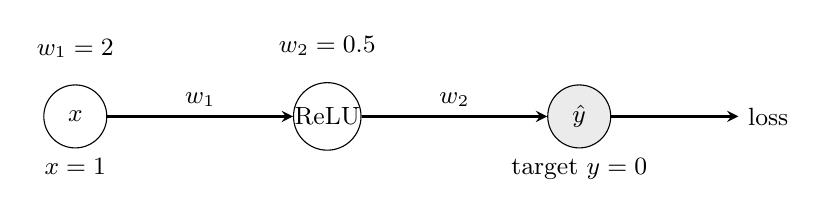
\begin{tikzpicture}[x=1.6cm, y=1cm,
  n/.style={circle, draw, minimum size=8mm, inner sep=0pt, font=\small}, >=stealth]
  \node[n] (x) at (0,0) {$x$};
  \node[n] (h) at (2,0) {ReLU};
  \node[n, fill=black!8] (y) at (4,0) {$\hat y$};
  \node[font=\small] (L) at (5.5,0) {loss};
  \draw[->, thick] (x)--node[above,font=\small]{$w_1$}(h);
  \draw[->, thick] (h)--node[above,font=\small]{$w_2$}(y);
  \draw[->, thick] (y)--(L);
  \node[below, font=\small] at (x.south) {$x=1$};
  \node[above=6pt, font=\small] at (x.north) {$w_1=2$};
  \node[above=6pt, font=\small] at (h.north) {$w_2=0.5$};
  \node[below, font=\small] at (y.south) {target $y=0$};
\end{tikzpicture}
\end{center}

\textbf{(a) Forward pass.}\; {\small Fill in each value, then square the error to get the loss.}
\begin{align*}
h &= \operatorname{ReLU}(w_1 \cdot x) = \operatorname{ReLU}(2 \times 1) = \rb{$2$}{1.4cm}
&\hat y &= w_2 \cdot h = 0.5 \times \rb{$2$}{1cm} = \rb{$1$}{1.4cm}\\[3pt]
\text{error} &= \hat y - y = \rb{$1$}{1.4cm}
&\text{loss} &= (\text{error})^2 = \rb{$1$}{1.4cm}
\end{align*}

\work{0.4cm}

\keybox{$h=\operatorname{ReLU}(2)=2$; \ $\hat y = 0.5\times 2 = 1$; \ error $=1-0=1$; \
loss $=1^2 = 1$. The guess overshot the target of $0$.}

\vspace{4pt}
\textbf{(b) Backward pass --- multiply the local effects along the path.}\;
{\small Recipe from lecture: start with the ``how wrong'' signal $=2\times\text{error}$, then
multiply the local effect at each arrow back to the weight. (The ReLU slope is $1$ because the
hidden value is positive.)}

\vspace{3pt}
``how wrong'' signal $= 2 \times \text{error} = 2 \times 1 = \rb{$2$}{1.4cm}$

\[
\text{gradient of } w_2 \;=\; (2\times\text{error}) \times h
\;=\; \blk{2.4cm} \;=\; \rb{$4$}{1.4cm}
\]
\[
\text{gradient of } w_1 \;=\; (2\times\text{error}) \times w_2 \times (\text{ReLU slope}) \times x
\;=\; \blk{3.6cm} \;=\; \rb{$1$}{1.4cm}
\]

\work{0.6cm}

\keybox{The shared ``how wrong'' signal is $2\times\text{error}=2\times 1 = 2$.\\
gradient of $w_2 = 2 \times h = 2 \times 2 = \mathbf{4}$ \ (short path: only the last weight).\\
gradient of $w_1 = 2 \times w_2 \times 1 \times x = 2 \times 0.5 \times 1 \times 1 = \mathbf{1}$
\ (longer path: back through $w_2$ and the ReLU). Both gradients are positive, so both weights
should decrease.}

\vspace{2pt}\hrule\vspace{5pt}

% =========================== Q2 ===========================
\textbf{2. One gradient-descent step by hand.}\; {\small Use your gradients from Q1 and the
update rule} $\text{new weight} = \text{weight} - \text{lr}\times\text{gradient}$, {\small with
learning rate lr $=0.1$.}

\[
w_2 \leftarrow 0.5 - 0.1 \times \rb{$4$}{1cm} = \rb{$0.1$}{1.6cm}
\qquad\qquad
w_1 \leftarrow 2 - 0.1 \times \rb{$1$}{1cm} = \rb{$1.9$}{1.6cm}
\]

\work{0.7cm}

\keybox{$w_2 \leftarrow 0.5 - 0.1\times 4 = 0.5 - 0.4 = \mathbf{0.1}$; \quad
$w_1 \leftarrow 2 - 0.1\times 1 = 2 - 0.1 = \mathbf{1.9}$. Both came down, as expected --- the
guess was too high. (Re-running the forward pass with the new weights gives loss $\approx 0.04$,
down from $1$: one step already helped.)}

\vspace{2pt}\hrule\vspace{5pt}

% =========================== Q3 ===========================
\textbf{3. Diagnose the loss curve --- and prescribe the fix.}\; {\small For each run, write the
\emph{diagnosis} and the \emph{one change} you would make, using the word banks. Each plot is loss
(vertical) vs.\ epoch (horizontal). Note that (a) and (d) are \textbf{not} the same problem.}

\vspace{4pt}
\begin{center}
\newcommand{\lossaxes}{\draw[->,gray] (0,0)--(3.1,0); \draw[->,gray] (0,0)--(0,2.4);}
%
\begin{minipage}[t]{0.235\linewidth}\centering
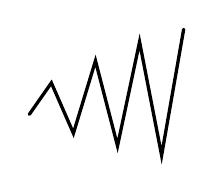
\begin{tikzpicture}[scale=0.8, line cap=round]
  \lossaxes
  \draw[very thick] (0.15,1.0)--(0.5,1.5)--(0.85,0.7)--(1.2,1.85)--(1.55,0.5)--(1.9,2.15)--(2.25,0.35)--(2.6,2.35);
\end{tikzpicture}\\[2pt]
{\footnotesize (a)}\\[3pt]
{\scriptsize diag:}\;\rb{far too high}{1.5cm}\\[4pt]
{\scriptsize fix:}\;\rb{lower a lot}{1.5cm}
\end{minipage}\hfill
%
\begin{minipage}[t]{0.235\linewidth}\centering
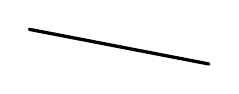
\begin{tikzpicture}[scale=0.8, line cap=round]
  \lossaxes
  \draw[very thick] (0.1,2.05)--(2.95,1.5);
\end{tikzpicture}\\[2pt]
{\footnotesize (b)}\\[3pt]
{\scriptsize diag:}\;\rb{too low}{1.5cm}\\[4pt]
{\scriptsize fix:}\;\rb{raise it}{1.5cm}
\end{minipage}\hfill
%
\begin{minipage}[t]{0.235\linewidth}\centering
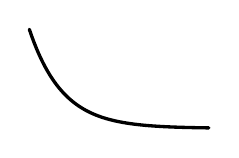
\begin{tikzpicture}[scale=0.8, line cap=round]
  \lossaxes
  \draw[very thick, samples=80, domain=0.1:2.95] plot (\x,{0.35+1.9*exp(-1.9*\x)});
\end{tikzpicture}\\[2pt]
{\footnotesize (c)}\\[3pt]
{\scriptsize diag:}\;\rb{just right}{1.5cm}\\[4pt]
{\scriptsize fix:}\;\rb{keep it}{1.5cm}
\end{minipage}\hfill
%
\begin{minipage}[t]{0.235\linewidth}\centering
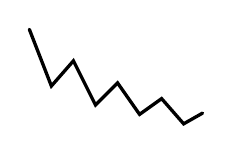
\begin{tikzpicture}[scale=0.8, line cap=round]
  \lossaxes
  \draw[very thick] (0.15,2.05)--(0.5,1.15)--(0.85,1.55)--(1.2,0.85)--(1.55,1.2)--(1.9,0.7)--(2.25,0.95)--(2.6,0.55)--(2.9,0.72);
\end{tikzpicture}\\[2pt]
{\footnotesize (d)}\\[3pt]
{\scriptsize diag:}\;\rb{a bit high}{1.5cm}\\[4pt]
{\scriptsize fix:}\;\rb{lower a little}{1.5cm}
\end{minipage}
\end{center}

\vspace{2pt}
\begin{center}
{\small \textbf{Diagnosis bank:}\;\; far too high (diverging) \;$\cdot$\; a bit too high (noisy but
converging) \;$\cdot$\; too low \;$\cdot$\; just right \\[2pt]
\textbf{Fix bank:}\;\; lower the rate a lot \;$\cdot$\; lower it a little \;$\cdot$\; raise it
\;$\cdot$\; keep it (train longer)}
\end{center}

\keybox{(a) \textbf{far too high $\rightarrow$ lower the rate a lot}: the swings \emph{grow} and the
loss climbs --- the steps overshoot so badly training is diverging. (b) \textbf{too low
$\rightarrow$ raise it}: the loss barely drops and is still high and still falling at the end;
it would get there eventually but wastes time. (c) \textbf{just right $\rightarrow$ keep it}: a
steep early drop that flattens out low and stays there. (d) \textbf{a bit too high $\rightarrow$
lower it a little}: the loss \emph{is} trending down but bounces noisily on the way --- close to
right, just overshooting slightly. The tell that separates (a) from (d): in (a) the swings grow
and the loss rises; in (d) they shrink and the loss falls.}

\vspace{2pt}\hrule\vspace{5pt}

% =========================== Q4 ===========================
\textbf{4. Spot the bug.}\; {\small A colleague's training loop runs with no error, but the loss
\emph{never drops} --- the weights never change at all. All five lines are present, in this order:}

\vspace{4pt}
\begin{center}
\begin{tabular}{@{}l@{\qquad}p{0.40\textwidth}@{}}
\texttt{for x, y in loader:}        & {\small\itshape every batch} \\[4pt]
\hspace{1em}\texttt{pred = model(x)}         & {\small\itshape forward} \\[4pt]
\hspace{1em}\texttt{loss = loss\_fn(pred, y)} & {\small\itshape how wrong?} \\[4pt]
\hspace{1em}\texttt{loss.backward()}          & {\small\itshape backprop the blame} \\[4pt]
\hspace{1em}\texttt{optimizer.zero\_grad()}   & {\small\itshape clear gradients} \\[4pt]
\hspace{1em}\texttt{optimizer.step()}         & {\small\itshape nudge every weight} \\
\end{tabular}
\end{center}

{\small (i) Which line is in the \textbf{wrong place}?}\; \rb{\texttt{optimizer.zero\_grad()}}{6cm}\\[4pt]
{\small (ii) Why does that stop learning, and where should it go?}

\work{0.5cm}

\keybox{(i) \texttt{optimizer.zero\_grad()} is misplaced --- it runs \emph{after}
\texttt{loss.backward()}. (ii) \texttt{backward()} computes this batch's gradients and stores them in
each weight's \texttt{.grad}; \texttt{zero\_grad()} then immediately \textbf{erases} them, so
\texttt{optimizer.step()} applies all-zero gradients and no weight moves --- the loss stays flat
forever. Move \texttt{zero\_grad()} to \emph{before} \texttt{backward()} (correct order:
\texttt{zero\_grad} $\rightarrow$ \texttt{backward} $\rightarrow$ \texttt{step}). Gradients live in
\texttt{.grad} and must be cleared just \emph{before}, never just after, the backward sweep.}

% =========================== Q5 ===========================
\textbf{5. Looking ahead (discussion).}\; {\small A short thought question --- one or two sentences
each. This one previews a later lecture, so reason it out rather than compute.}

\vspace{3pt}
You train a network and watch the loss on your \emph{training} samples fall steadily, almost to
zero --- the model gets the training data nearly perfect. But when you score it on a batch of
\emph{fresh, held-out} samples it has never seen, the loss stops improving and then starts to
\emph{rise}.

\vspace{4pt}
(a) What might be going wrong? \hfill (b) Does a lower training loss always mean a better model?

\work{1.6cm}
\ifsolution\else\blk{\linewidth}\\[10pt]\blk{\linewidth}\\[10pt]\blk{\linewidth}\fi

\keybox{(a) This is \textbf{overfitting}: the network is starting to \emph{memorise} the quirks and
noise of the training set instead of learning the general pattern, so it keeps improving on seen
data while getting worse on new data. (b) \textbf{No.} A lower \emph{training} loss does not mean a
better model --- what matters is performance on \emph{unseen} data (generalisation); once the two
curves split apart, more training makes the model worse in practice. (Lecture 4 names the fixes:
more/cleaner data, regularisation, dropout, and early stopping --- stop where the held-out loss
turns up.)}

\vspace{4pt}\hrule\vspace{3pt}
{\small\itshape \ifsolution Answer key.\else Keep this sheet --- the backprop recipe and the
five-line loop are your Lab 1 cheat-sheet.\fi}

\end{document}
"
%  (or, to flip by hand, change \solutionfalse to \solutiontrue below.)
% =====================================================================
\documentclass[11pt]{article}

\newif\ifsolution
\ifdefined\showsolutions \solutiontrue \else \solutionfalse \fi
% \solutiontrue   % <-- uncomment to hard-code the ANSWER KEY build

\usepackage[letterpaper, margin=0.6in, top=0.7in, bottom=0.5in]{geometry}
\usepackage{amsmath, amssymb}
\usepackage{xcolor}
\usepackage{tikz}
\usepackage{fancyhdr}

\pagestyle{fancy}
\fancyhf{}
\fancyhead[L]{\small\textbf{MSACL DS301 --- Deep Learning}}
\fancyhead[R]{\small\textbf{Quiz 2: How Networks Learn\ifsolution\ \textmd{(Answer Key)}\fi}}
\fancyfoot[C]{\thepage}
\renewcommand{\headrulewidth}{0.4pt}

\newcommand{\blk}[1]{\underline{\hspace{#1}}}
% Reveal-or-blank: shows the answer in the key, a blank rule on the student sheet.
\newcommand{\rb}[2]{\ifsolution\textbf{#1}\else\blk{#2}\fi}
% Boxed answer (key only) and blank writing space (student only).
\newcommand{\keybox}[1]{\ifsolution\par\vspace{2pt}%
  \fbox{\parbox{0.965\textwidth}{\small\textbf{Answer.}\; #1}}\par\fi}
\newcommand{\work}[1]{\ifsolution\else\vspace{#1}\fi}

\setlength{\parindent}{0pt}
\setlength{\parskip}{3pt}
\setlength{\abovedisplayskip}{5pt}
\setlength{\belowdisplayskip}{5pt}

\begin{document}

\begin{center}
{\Large \textbf{Quiz 2 --- How Networks Learn}}\\[2pt]
{\normalsize Loss, backpropagation, one gradient-descent step, and the training loop}
\end{center}

\vspace{-2pt}
\begin{center}
\fbox{\parbox{0.92\textwidth}{\small
\textbf{Instructions:}\; Answer all five questions. Intuition first, light arithmetic ---
show your work on the blanks. No calculators needed.%
\ifsolution\else\\[4pt]\textbf{Name:}\ \blk{6cm}\hfill\textbf{Date:}\ \blk{3.5cm}\fi
}}
\end{center}

\vspace{-2pt}\hrule\vspace{5pt}

% =========================== Q1 ===========================
\textbf{1. Backpropagation on a two-weight network.}\; {\small Same tiny net as the worked
example: one input, one hidden neuron (ReLU), one output --- just two weights.}

\vspace{2pt}
\begin{center}
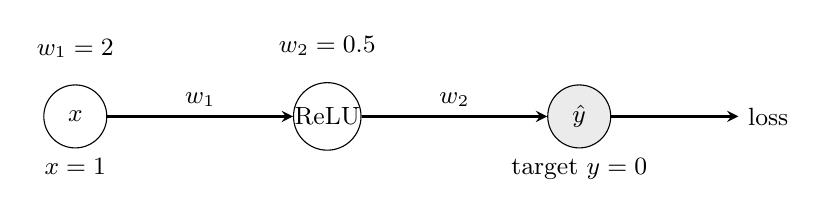
\begin{tikzpicture}[x=1.6cm, y=1cm,
  n/.style={circle, draw, minimum size=8mm, inner sep=0pt, font=\small}, >=stealth]
  \node[n] (x) at (0,0) {$x$};
  \node[n] (h) at (2,0) {ReLU};
  \node[n, fill=black!8] (y) at (4,0) {$\hat y$};
  \node[font=\small] (L) at (5.5,0) {loss};
  \draw[->, thick] (x)--node[above,font=\small]{$w_1$}(h);
  \draw[->, thick] (h)--node[above,font=\small]{$w_2$}(y);
  \draw[->, thick] (y)--(L);
  \node[below, font=\small] at (x.south) {$x=1$};
  \node[above=6pt, font=\small] at (x.north) {$w_1=2$};
  \node[above=6pt, font=\small] at (h.north) {$w_2=0.5$};
  \node[below, font=\small] at (y.south) {target $y=0$};
\end{tikzpicture}
\end{center}

\textbf{(a) Forward pass.}\; {\small Fill in each value, then square the error to get the loss.}
\begin{align*}
h &= \operatorname{ReLU}(w_1 \cdot x) = \operatorname{ReLU}(2 \times 1) = \rb{$2$}{1.4cm}
&\hat y &= w_2 \cdot h = 0.5 \times \rb{$2$}{1cm} = \rb{$1$}{1.4cm}\\[3pt]
\text{error} &= \hat y - y = \rb{$1$}{1.4cm}
&\text{loss} &= (\text{error})^2 = \rb{$1$}{1.4cm}
\end{align*}

\work{0.4cm}

\keybox{$h=\operatorname{ReLU}(2)=2$; \ $\hat y = 0.5\times 2 = 1$; \ error $=1-0=1$; \
loss $=1^2 = 1$. The guess overshot the target of $0$.}

\vspace{4pt}
\textbf{(b) Backward pass --- multiply the local effects along the path.}\;
{\small Recipe from lecture: start with the ``how wrong'' signal $=2\times\text{error}$, then
multiply the local effect at each arrow back to the weight. (The ReLU slope is $1$ because the
hidden value is positive.)}

\vspace{3pt}
``how wrong'' signal $= 2 \times \text{error} = 2 \times 1 = \rb{$2$}{1.4cm}$

\[
\text{gradient of } w_2 \;=\; (2\times\text{error}) \times h
\;=\; \blk{2.4cm} \;=\; \rb{$4$}{1.4cm}
\]
\[
\text{gradient of } w_1 \;=\; (2\times\text{error}) \times w_2 \times (\text{ReLU slope}) \times x
\;=\; \blk{3.6cm} \;=\; \rb{$1$}{1.4cm}
\]

\work{0.6cm}

\keybox{The shared ``how wrong'' signal is $2\times\text{error}=2\times 1 = 2$.\\
gradient of $w_2 = 2 \times h = 2 \times 2 = \mathbf{4}$ \ (short path: only the last weight).\\
gradient of $w_1 = 2 \times w_2 \times 1 \times x = 2 \times 0.5 \times 1 \times 1 = \mathbf{1}$
\ (longer path: back through $w_2$ and the ReLU). Both gradients are positive, so both weights
should decrease.}

\vspace{2pt}\hrule\vspace{5pt}

% =========================== Q2 ===========================
\textbf{2. One gradient-descent step by hand.}\; {\small Use your gradients from Q1 and the
update rule} $\text{new weight} = \text{weight} - \text{lr}\times\text{gradient}$, {\small with
learning rate lr $=0.1$.}

\[
w_2 \leftarrow 0.5 - 0.1 \times \rb{$4$}{1cm} = \rb{$0.1$}{1.6cm}
\qquad\qquad
w_1 \leftarrow 2 - 0.1 \times \rb{$1$}{1cm} = \rb{$1.9$}{1.6cm}
\]

\work{0.7cm}

\keybox{$w_2 \leftarrow 0.5 - 0.1\times 4 = 0.5 - 0.4 = \mathbf{0.1}$; \quad
$w_1 \leftarrow 2 - 0.1\times 1 = 2 - 0.1 = \mathbf{1.9}$. Both came down, as expected --- the
guess was too high. (Re-running the forward pass with the new weights gives loss $\approx 0.04$,
down from $1$: one step already helped.)}

\vspace{2pt}\hrule\vspace{5pt}

% =========================== Q3 ===========================
\textbf{3. Diagnose the loss curve --- and prescribe the fix.}\; {\small For each run, write the
\emph{diagnosis} and the \emph{one change} you would make, using the word banks. Each plot is loss
(vertical) vs.\ epoch (horizontal). Note that (a) and (d) are \textbf{not} the same problem.}

\vspace{4pt}
\begin{center}
\newcommand{\lossaxes}{\draw[->,gray] (0,0)--(3.1,0); \draw[->,gray] (0,0)--(0,2.4);}
%
\begin{minipage}[t]{0.235\linewidth}\centering
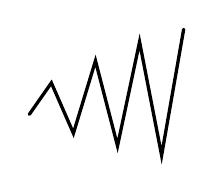
\begin{tikzpicture}[scale=0.8, line cap=round]
  \lossaxes
  \draw[very thick] (0.15,1.0)--(0.5,1.5)--(0.85,0.7)--(1.2,1.85)--(1.55,0.5)--(1.9,2.15)--(2.25,0.35)--(2.6,2.35);
\end{tikzpicture}\\[2pt]
{\footnotesize (a)}\\[3pt]
{\scriptsize diag:}\;\rb{far too high}{1.5cm}\\[4pt]
{\scriptsize fix:}\;\rb{lower a lot}{1.5cm}
\end{minipage}\hfill
%
\begin{minipage}[t]{0.235\linewidth}\centering
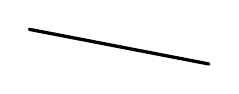
\begin{tikzpicture}[scale=0.8, line cap=round]
  \lossaxes
  \draw[very thick] (0.1,2.05)--(2.95,1.5);
\end{tikzpicture}\\[2pt]
{\footnotesize (b)}\\[3pt]
{\scriptsize diag:}\;\rb{too low}{1.5cm}\\[4pt]
{\scriptsize fix:}\;\rb{raise it}{1.5cm}
\end{minipage}\hfill
%
\begin{minipage}[t]{0.235\linewidth}\centering
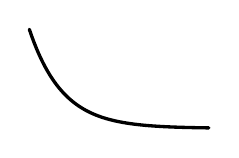
\begin{tikzpicture}[scale=0.8, line cap=round]
  \lossaxes
  \draw[very thick, samples=80, domain=0.1:2.95] plot (\x,{0.35+1.9*exp(-1.9*\x)});
\end{tikzpicture}\\[2pt]
{\footnotesize (c)}\\[3pt]
{\scriptsize diag:}\;\rb{just right}{1.5cm}\\[4pt]
{\scriptsize fix:}\;\rb{keep it}{1.5cm}
\end{minipage}\hfill
%
\begin{minipage}[t]{0.235\linewidth}\centering
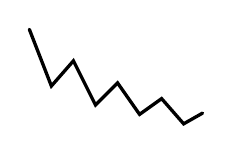
\begin{tikzpicture}[scale=0.8, line cap=round]
  \lossaxes
  \draw[very thick] (0.15,2.05)--(0.5,1.15)--(0.85,1.55)--(1.2,0.85)--(1.55,1.2)--(1.9,0.7)--(2.25,0.95)--(2.6,0.55)--(2.9,0.72);
\end{tikzpicture}\\[2pt]
{\footnotesize (d)}\\[3pt]
{\scriptsize diag:}\;\rb{a bit high}{1.5cm}\\[4pt]
{\scriptsize fix:}\;\rb{lower a little}{1.5cm}
\end{minipage}
\end{center}

\vspace{2pt}
\begin{center}
{\small \textbf{Diagnosis bank:}\;\; far too high (diverging) \;$\cdot$\; a bit too high (noisy but
converging) \;$\cdot$\; too low \;$\cdot$\; just right \\[2pt]
\textbf{Fix bank:}\;\; lower the rate a lot \;$\cdot$\; lower it a little \;$\cdot$\; raise it
\;$\cdot$\; keep it (train longer)}
\end{center}

\keybox{(a) \textbf{far too high $\rightarrow$ lower the rate a lot}: the swings \emph{grow} and the
loss climbs --- the steps overshoot so badly training is diverging. (b) \textbf{too low
$\rightarrow$ raise it}: the loss barely drops and is still high and still falling at the end;
it would get there eventually but wastes time. (c) \textbf{just right $\rightarrow$ keep it}: a
steep early drop that flattens out low and stays there. (d) \textbf{a bit too high $\rightarrow$
lower it a little}: the loss \emph{is} trending down but bounces noisily on the way --- close to
right, just overshooting slightly. The tell that separates (a) from (d): in (a) the swings grow
and the loss rises; in (d) they shrink and the loss falls.}

\vspace{2pt}\hrule\vspace{5pt}

% =========================== Q4 ===========================
\textbf{4. Spot the bug.}\; {\small A colleague's training loop runs with no error, but the loss
\emph{never drops} --- the weights never change at all. All five lines are present, in this order:}

\vspace{4pt}
\begin{center}
\begin{tabular}{@{}l@{\qquad}p{0.40\textwidth}@{}}
\texttt{for x, y in loader:}        & {\small\itshape every batch} \\[4pt]
\hspace{1em}\texttt{pred = model(x)}         & {\small\itshape forward} \\[4pt]
\hspace{1em}\texttt{loss = loss\_fn(pred, y)} & {\small\itshape how wrong?} \\[4pt]
\hspace{1em}\texttt{loss.backward()}          & {\small\itshape backprop the blame} \\[4pt]
\hspace{1em}\texttt{optimizer.zero\_grad()}   & {\small\itshape clear gradients} \\[4pt]
\hspace{1em}\texttt{optimizer.step()}         & {\small\itshape nudge every weight} \\
\end{tabular}
\end{center}

{\small (i) Which line is in the \textbf{wrong place}?}\; \rb{\texttt{optimizer.zero\_grad()}}{6cm}\\[4pt]
{\small (ii) Why does that stop learning, and where should it go?}

\work{0.5cm}

\keybox{(i) \texttt{optimizer.zero\_grad()} is misplaced --- it runs \emph{after}
\texttt{loss.backward()}. (ii) \texttt{backward()} computes this batch's gradients and stores them in
each weight's \texttt{.grad}; \texttt{zero\_grad()} then immediately \textbf{erases} them, so
\texttt{optimizer.step()} applies all-zero gradients and no weight moves --- the loss stays flat
forever. Move \texttt{zero\_grad()} to \emph{before} \texttt{backward()} (correct order:
\texttt{zero\_grad} $\rightarrow$ \texttt{backward} $\rightarrow$ \texttt{step}). Gradients live in
\texttt{.grad} and must be cleared just \emph{before}, never just after, the backward sweep.}

% =========================== Q5 ===========================
\textbf{5. Looking ahead (discussion).}\; {\small A short thought question --- one or two sentences
each. This one previews a later lecture, so reason it out rather than compute.}

\vspace{3pt}
You train a network and watch the loss on your \emph{training} samples fall steadily, almost to
zero --- the model gets the training data nearly perfect. But when you score it on a batch of
\emph{fresh, held-out} samples it has never seen, the loss stops improving and then starts to
\emph{rise}.

\vspace{4pt}
(a) What might be going wrong? \hfill (b) Does a lower training loss always mean a better model?

\work{1.6cm}
\ifsolution\else\blk{\linewidth}\\[10pt]\blk{\linewidth}\\[10pt]\blk{\linewidth}\fi

\keybox{(a) This is \textbf{overfitting}: the network is starting to \emph{memorise} the quirks and
noise of the training set instead of learning the general pattern, so it keeps improving on seen
data while getting worse on new data. (b) \textbf{No.} A lower \emph{training} loss does not mean a
better model --- what matters is performance on \emph{unseen} data (generalisation); once the two
curves split apart, more training makes the model worse in practice. (Lecture 4 names the fixes:
more/cleaner data, regularisation, dropout, and early stopping --- stop where the held-out loss
turns up.)}

\vspace{4pt}\hrule\vspace{3pt}
{\small\itshape \ifsolution Answer key.\else Keep this sheet --- the backprop recipe and the
five-line loop are your Lab 1 cheat-sheet.\fi}

\end{document}
